\documentclass[12pt,a4paper, oneside]{article}
\usepackage[utf8]{inputenc}
\usepackage[T1]{fontenc}
\usepackage[english,german]{babel}
\usepackage[style=german]{csquotes}
\usepackage{graphicx}

\author{Uni Oldenburg, SWP2020 Gruppe A}
\begin{document}
\begin{titlepage}
\pagestyle{empty}
\begin{center}

\begin{figure}[h]									
\centering											

\includegraphics[width=0.35\textwidth]{../img/Logo.jpg}
\end{figure}		

\bigskip \bigskip \noindent							
\textsc{\textbf{\LARGE Softwareprojekt:}} \par \bigskip \noindent																			
\textsc{\textbf{\LARGE Projekttagebuch}} 			    
													
\par \bigskip \bigskip \bigskip \bigskip \bigskip \noindent
{\Large Gruppe A} \par \medskip \noindent
		
\par \bigskip \bigskip \bigskip \bigskip \bigskip \bigskip \noindent																		
\textit{\Large Wintersemester 2020/21 und} \par \noindent
\textit{\Large Sommersemester 2021}				
													
\par \bigskip \bigskip \bigskip \bigskip \bigskip \bigskip \noindent			
\par \bigskip \bigskip \bigskip \noindent
{\Large Sprintanalyse} \par \medskip \noindent
		
\end{center}
\end{titlepage}

\tableofcontents
\pagebreak

\section{Sprinttagebuch: Sprint-Nr. 8}
\underline{Name des Sprints:}
\\
Sprint 8: The Adventure Begins

\noindent
\\
\underline{Zeitraum des Sprints:} 
\\
01. April 2021 - 13. März 2021

\noindent 
\\
\underline{Ziel des Sprints:} 
\\
Eine Partie Catan soll spielbar sein

\noindent
\\
\underline {Team:} 
\\
Sven Ahrens, Alwin Bossert, Aldin Dervisi, Marvin Drees, Mario Fokken,
Timo Gerken, Finn Haase, Temmo Junkhoff, Maximilian Lindner, Steven Luong, Phillip-André Suhr, Eric Vuong


\section{Vorgänge}

\begin{itemize}

\item SWP2020A-130: ANmi Siedlungen, Städte und Straßen bauen können (4 Story Points)

\item SWP2020A-140: ANmi, dass die Längste Handelsstraße und Größte Rittermacht automatisch korrekt zugewiesen werden (2 Story Points)

\item SWP2020A-196:	ANmi, wenn ich einen bestimmten Hafen besitze, dessen Wechselkurs bei der Bank nutzen können (2 Story Points)

\item SWP2020A-198:	ANmi, dass der Räuber entsprechend den Regeln Ressourcen stiehlt und Felder blockiert (3 Story Points)

\item SWP2020A-220:	Bericht für Sprint 7 erstellen (2 Story Points)

\item SWP2020A-227:	ANmi bei Client-Wechsel den vorherigen Lobbys/Spielen beitreten (2 Story Points)

\item SWP2020A-241: ANmi über einen Button im Hauptmenü einer zufälligen Lobby beitreten können (1 Story Point)

\item SWP2020A-244: Behandlung der Exceptions/ExceptionMessages verbessern (3 Story Points)

\item SWP2020A-247: ResourceBundle-Maintenance (1 Story Point)

\item SWP2020A-250: GetUserSessionEvent in AuthenticationService verlagern und besser benennen (1 Story Point)

\item SWP2020A-251:	Den aktuell eingeloggten User auf Clientseite im Userservice speichern, um ihn nicht mehr hacky zu jedem Presenter durchreichen zu müssen (2 Story Points)

\item SWP2020A-252:	Die Überprüfung der Siegpunkte sollte auf Serverseite ausgelöst werden (1 Story Point)

\item SWP2020A-253:	ANmi ich eine Beschriftung diverser UI Elemente haben (1 Story Point)

\item SWP2020A-254:	ANmi meine Accountdetails nicht ändern können während ich mich in einer Lobby befinde (1 Story Point)

\item SWP2020A-257: 6500\%-Warnung bei Clientstart beheben (1 Story Point)

\item SWP2020A-258:	SessionManagement \& SessionStore erstellen als Single Point of Truth für Session-Objekte (3 Story Points)

\item SWP2020A-259:	KickUser- und StartSession-Buttons sind während einer Partie sichtbar (1 Story Point)

\item SWP2020A-260:	ChangeAccountDetails-Fenster soll bei Klick auf X / Alt+F4 nur ins Hauptmenü gehen (2 Story Points)

\item SWP2020A-262:	Dimensionskonstanten als public static final in Presenterklassen verlagern (1 Story Point)

\item SWP2020A-263: IUserManagement.getUserWithPassword(String, String) refactoren zu IUserManagement.getUser(String, String) (1 Story Point)

\item SWP2020A-264: Spielbezogene Methoden vom (Client-)LobbyService in neuen GameService verlagern (1 Story Point)

\end{itemize}

\newpage
\subsection{Sprinterfolg}
\begin{figure}[h]
    \centering
    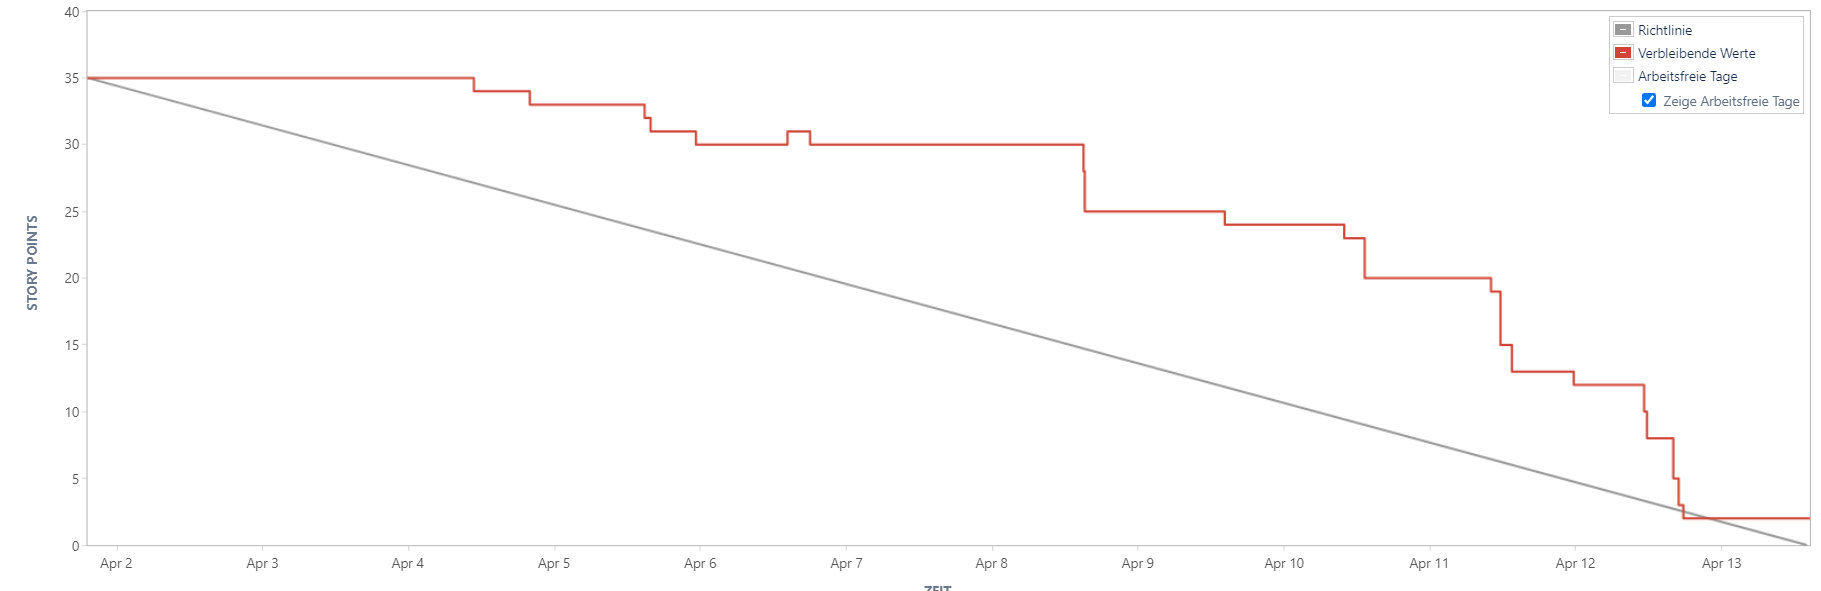
\includegraphics[width=\textwidth, height=5cm]{../img/sprint_08/Burndown-Sprint 8.PNG}
    \caption{Burndown-Diagramm Sprint 8}
    \label{fig: Burndown-Sprint 8}
\end{figure}
\noindent
Dieser Sprint war bisher der kleinste Sprint im Bezug auf die Höhe der Story Points im Verlauf des Software-Projektes und betrug einen Gesamtaufwand von 35 Story Points, weshalb der Sprintzeitraum dementsprechend auf eineinhalb Wochen gekürzt wurde.
Aus dem Burndown-Diagramm wird ersichtlich, dass im frühem Verlauf des Sprints die Arbeitsaktivität eher gering war, wobei jedoch im mittleren Zeitraum die Aktivität deutlich gestiegen ist, was ersichtlich ist aufgrund dessen, dass viele Vorgänge im mittlerem Zeitraum bereits in PR gestellt wurden.
In diesem Sprint war erstmals eine Anzahl von 9 PR´s gleichzeitig offen für Reviews. Des Weiteren wurde folgende Task nachgezogen: \textit{SWP2020A-264: Spielbezogene Methoden vom (Client-)LobbyService in neuen GameService verlagern (1 Story Point)}, wobei folglich unser Sprintaufwand von 35 Story Points auf 36 Story Points erhöht wurde.
Schlussendlich wurden alle Vorgänge bis auf die Task: \textit{SWP2020A-140: ANmi, dass die Längste Handelsstraße und Größte Rittermacht automatisch korrekt zugewiesen werden (2 Story Points)} am 14. April 2021 erfolgreich abgeschlossen und eine Gesamtanzahl von 34 Story Points abgeschlossen.

\newpage
\subsection{Sprintprobleme bzw. Hindernisse}
Zum Anfang des Sprints am 01. April 2021 bis hin zum 04. April 2021 hatte das Team keinerlei Fortschritt vorgewiesen im Bezug auf abgeschlossene Tasks.
Weiterhin wurde in diesem Sprint ersichtlich, dass einige Reviews definitv zu lang gebraucht haben und infolgedessen viele Tasks bzw. PR´s lange in Review standen.
Dies führte dementsprechend auch zur einer erhöhten Ansammlung von PR´s in Git bzw. Bitbucket und einem niedrigen Abschlussverzeichnis im Burndown-Diagramm.
Ein weiteres Problem war das gegenseitige Blockieren von Tasks, wobei viele Vorgänge nicht richtig getestet werden konnten, aufgrund dessen Abhängigkeit von anderen Task, die noch in Bearbeitung waren.
Beispielweise konnte der Vorgang \textit{ (SWP2020A-140: ANmi, dass die Längste Handelsstraße und Größte Rittermacht automatisch korrekt zugewiesen werden)} nicht richtig getestet werden, da sie teils abhängig war von der Task: \textit{SWP2020A-130: ANmi Siedlungen, Städte und Straßen bauen können}.
Des Weiteren wurde in diesem Sprint die Task: \textit{SWP2020A-140: ANmi, dass die Längste Handelsstraße und Größte Rittermacht automatisch korrekt zugewiesen werden (2 Story Points)} nicht abgeschlossen aufgrund eines Problems bei der Berechnung der längsten Handelsstraße.
Die Task war zwar bereits in PR, jedoch wurde sie aufgrund zeitlichen Gründen in den nächsten Sprint verlagert.


\section{Erkenntnis aus der Retrospektive}
Folgende Erkenntnisse ergaben sich aus der Retrospektive:\\

\underline{Start:}
\begin{itemize}
    \item Reviews früher machen
    \item Reviewer ersetzen nach 72h und in den letzten 12h vor dem Reviewfreeze
\end{itemize}

\underline{Stop:}
\begin{itemize}
    \item Reviews hinauszögern bzw. Reviews brauchen zu lange
    \item Pair-Programming bzw. Reduzieren
\end{itemize}

\underline{Weiter so:}
\begin{itemize}
    \item Auf Discord ansprechbar sein (max. 2 Tage für Antworten)
\end{itemize}

\newpage
\section{Sonstige Anmerkungen}
Was grundsätzlich anzumerken war in diesem Sprint sind relativ langsame Reviews und die folgliche Anstauung von PR´s.
Außerdem die starke Reduzierung von Pair-Programming nach Feedback von unserem Tutor Roman, was für uns relativ bedauerlich war, da in jeder Retrospektive das Pair-Programming als besonders hilfreich und gut empfunden wurde.
Des Weiteren ist jedoch das Anbieten bzw. die Nachfrage nach Hilfe weiterhin möglich und auch erwünscht, sollte eine Person auf Probleme stoßen, die er vorerst allein nicht bewältigen kann.

\section{Fazit}
Generell lässt sich sagen, dass unser Sprintziel, eine Runde Catan zu spielen nicht vollständig erreicht wurde, da der Vorgang: \textit{SWP2020A-140: ANmi, dass die Längste Handelsstraße und Größte Rittermacht automatisch korrekt zugewiesen werden (2 Story Points)} nicht zum Sprintende abgeschlossen werden konnte.
Jedoch sind grundsätzlich alle Apsekte, um eine Runde Catan zu spielen bis auf die Task SWP2020A-140 vorhanden bzw. erfüllt.
Anschließend ist ersichtlich, dass nach dem nächsten Sprint, das Sprintziel defintiv erfüllt werden sein sollte.

\end{document}
